\documentclass{beamer}
\usetheme{Warsaw}  %% Themenwahl
\usepackage{commath}
\usepackage{subfig}
\usepackage[utf8]{inputenc}
\usepackage[T1]{fontenc}
\usepackage[UKenglish]{babel}


\title{Energy-efficient Routing Protocols for Mobile Ad-hoc Networks}
\author{Julian Andres Klode}
\date{March 1, 2016}

\begin{document}
\maketitle


\section{Introduction}
\frame{\tableofcontents[currentsection]}
\begin{frame}{Types of Mobile-Ad-hoc networks}
  \begin{Definition}[ad-hoc network]
    A wireless network of mobile nodes without base stations.
  \end{Definition}
  \begin{Definition}[mesh network]
    A ad-hoc network where all nodes take part in routing messages
  \end{Definition}
\end{frame}
\begin{frame}{Motivation}
  Use cases:

  \begin{itemize}
      \item Wireless sensor networks
      \item Internet-of-thing devices
      \item Mobile phones connecting directly with each others
  \end{itemize}

  and more.
\end{frame}


\begin{frame}{Power aware routing}
\begin{block}{Minimize active communication energy}
    Do one of:
    \begin{itemize}
        \item Power control -- Find the path with the smallest power consumption.
        \item Load distribution -- Choose paths based on the energy levels of the nodes
    \end{itemize}
    or do both!
\end{block}
\begin{block}{Sleep/power-down}
    Put unused nodes to sleep
\end{block}
(Yu, Lee, Youn\cite{main1})
\end{frame}
\begin{frame}{Other categories}
\begin{itemize}
    \item Proactive/table-driven
    \item Reactive/on-demand
    \item Hybrid proactive/reactive
    \item Geographical
    \item Multicast
    \item Geo-cast
    \item Multi-path
    \item Hierarchical
    \item Flow-oriented
    \item Mesh routing
\end{itemize}
    (Alotaibi and Mukherjee\cite{alotaibi2012survey})
\end{frame}

\section{Survey}
\frame{\tableofcontents[currentsection]}
\begin{frame}{Overview}
\begin{figure}
  \centering
  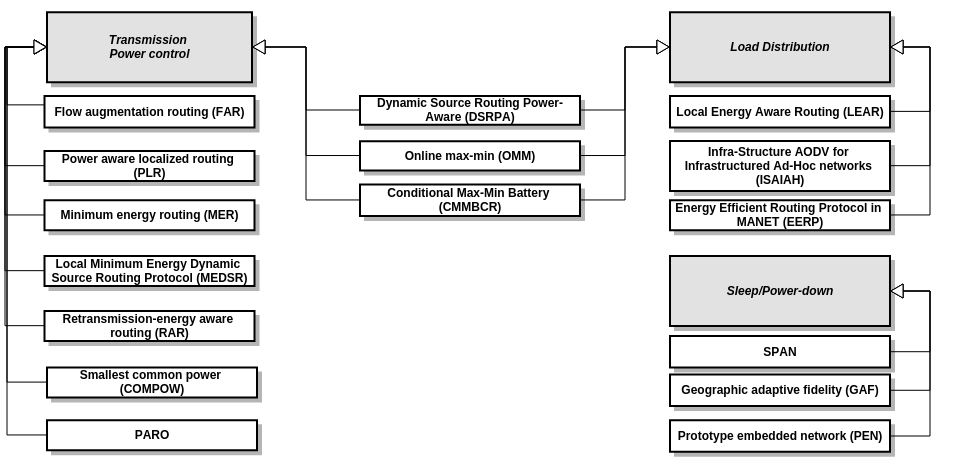
\includegraphics[width=0.9\textwidth]{images/overview}
  \caption{Overview of the protocols}
  
\end{figure}
\end{frame}
\subsection{Power control}
\begin{frame}{Flow augmentation routing (FAR)\cite{chang2000energy}}
    Finds the path with the minimum sum link cost
\begin{figure}
\centering
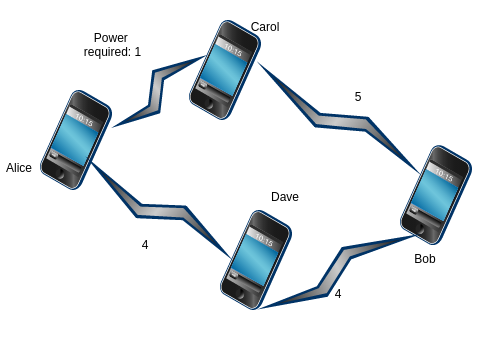
\includegraphics[width=0.5\textwidth]{images/far}
\caption{Simple routing example}
\end{figure}
\end{frame}
\begin{frame}{Power aware localized routing (PLR)\cite{stojmenovic2001power}}
    \begin{itemize}
        \item Power grows more than quadratic relative to distance
        \item Use geographical locations of source and destination to estimate required transmission power
        \item Each hop $A$ selects next hop $N$ based on power $p(\abs{AN})$ required to reach it and
              the power needed for an indirect transmission $q(\abs{ND})$ from that next hop to destination
    \end{itemize}
\begin{figure}
\centering
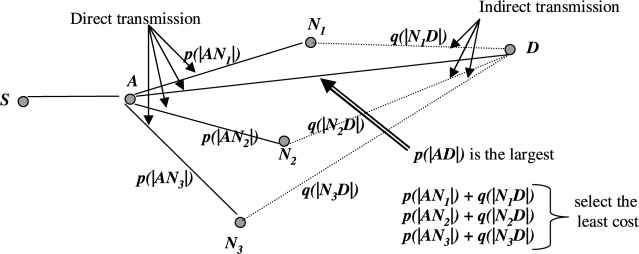
\includegraphics[width=0.6\textwidth]{images/plr-example}
\caption{Selection of next hop in PLR\cite{alotaibi2012survey}}
\label{plrexample}
\end{figure}
\end{frame}
\begin{frame}{Minimum energy routing (MER)}

\begin{table}[b]
  \begin{tabular}{ll}
    Options & Implementation Level  \\
    \hline
    A: Routing packet-based power control & Routing software/\\ &802.11 firmware \\
    B: Minimum energy routing & Routing software \\
    C: Cache replies off & Routing software \\
    D: Internal cache options & Routing software \\
    E: Multi-hop route discovery & Routing software \\
    F: MAC layer ACK power control & 802.11 firmware \\
    G: Route Maintenance with power sensing & Routing software \\
    H: HMAC-Level snooping and gratious replies & 802.11 firmware \\
  \end{tabular}
  \caption{Options in MER\cite{doshi2002demand}}
  \label{tbl:mer-options}
\end{table}
\end{frame}

\begin{frame}{Minimum energy routing (MER)}
\begin{block}{Option A, F: power control}
    \begin{itemize}
    \item Option A: Routing packet-based
    \begin{itemize}
        \item Append transmission power at each node in \textit{route-request} packets
        \item Send back in \textit{route-reply} packet
    \end{itemize}
    \item Option F: Same for packets in the MAC layer
    \end{itemize}
\end{block}
\begin{block}{Option B: Minimum energy routing}
    \begin{itemize}
        \item Find least energy route from cache and route using that
    \end{itemize}
\end{block}
\end{frame}

\begin{frame}{Minimum energy routing (MER)}
    \begin{block}{Option G: Route Maintenance with power sensing \& Routing software}
    \begin{itemize}
        \item Adjust routes for moving nodes
    \end{itemize}
\end{block}

\begin{block}{Option E, H: Multi-hop route discovery \& HMAC-level snooping and gratious replies}
    \begin{itemize}
        \item Discover alternative routes
        \item Advertise alternative more power efficient routes
    \end{itemize}
\end{block}
\end{frame}

\begin{frame}{Local Minimum Energy Dynamic Source Routing Protocol (MEDSR)\cite{tanque2007minimum}}
    \begin{itemize}
        \item Two power levels: Low and high
        \item Only single power-level field in packet
    \end{itemize}
    Example: Let low=2, high=4.
    \begin{figure}
\centering
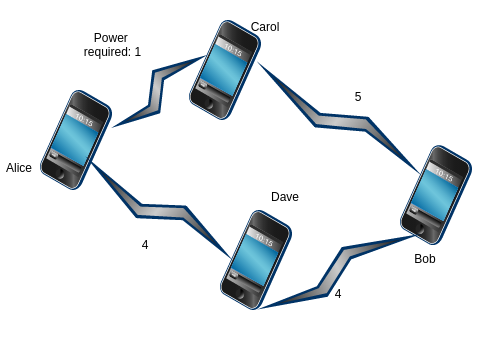
\includegraphics[width=0.45\textwidth]{images/far}
\caption{Simple routing example}
\end{figure}
\end{frame}

\begin{frame}{RAR and COMPOW}
\begin{block}{Retransmission-energy aware routing (RAR)\cite{banerjee2002minimum}}
    \begin{itemize}
        \item Modify link cost (expected required transmission power) to account for retransmissions: \\
        $\rightarrow$ multiply with expected number of tries
    \end{itemize}
\end{block}
\begin{block}{Smallest common power (COMPOW)\cite{narayanaswamy2002power}}
    \begin{itemize}
        \item Want to have bidirectional communication\\
            $\rightarrow$ define a smallest common power, so that all nodes can reach other other
    \end{itemize}
\end{block}
\end{frame}
\begin{frame}{COMPOW (continuation)}
\begin{figure}
\centering
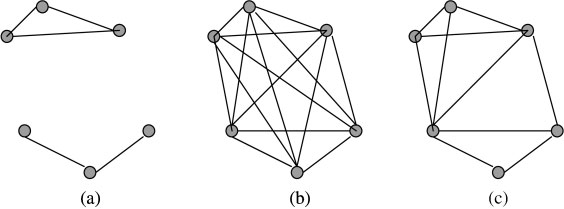
\includegraphics[width=0.7\textwidth]{images/compow-level-choice}
\caption{Power choice in COMPOW: (a) too low, (b) too high, (c) optimal}
\label{compow:power-choice}
\end{figure}
\end{frame}

\begin{frame}{PARO\cite{gomez2003paro}}
\begin{block}{Idea: Introduce intermediate nodes into a route}
    Shorter links $\rightarrow$ reduced power consumption
\end{block}
\begin{block}{Implementation}
\begin{itemize}
    \item When sending, Store transmission power in data packets
    \item Overhear transmission by other nodes and store estimated power to transmit to the other node
    \item When overhearing a transmission, send a \textit{route-redirect} message to source and destination,
          advertising that routing through your node is more energy efficient.
\end{itemize}
\end{block}
\end{frame}

\subsection{Load distribution}
\begin{frame}{Recap: Overview}
\begin{figure}
  \centering
  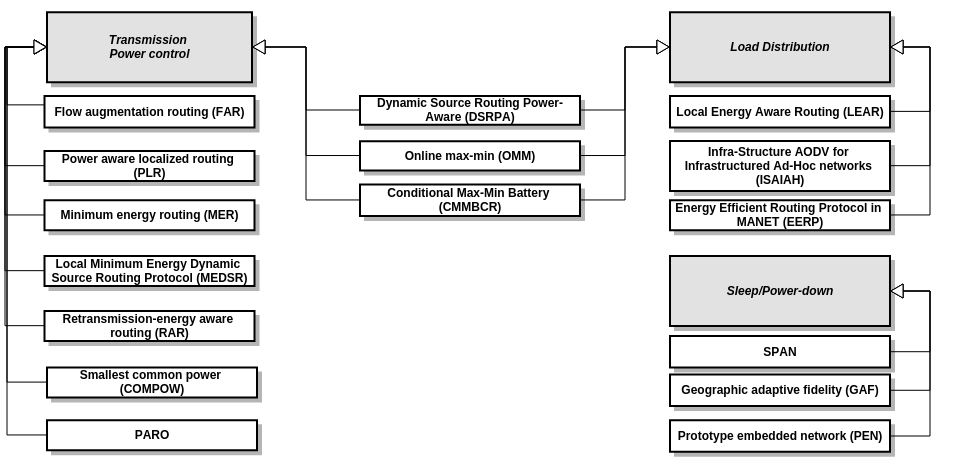
\includegraphics[width=0.9\textwidth]{images/overview}
  \caption{Overview of the protocols}
  
\end{figure}
\end{frame}
\begin{frame}{Local Energy Aware Routing Protocol (LEAR)\cite{woo2001non}}

\begin{block}{Route discovery}
\begin{itemize}
    \item Only forward route request messages if current power level above a threshold
    \item Threshold is defined locally, and decreases with battery level
    \item Lower threshold when receiving route request multiple times
\end{itemize}
\end{block}
\begin{block}{Route caching}
    \begin{itemize}
        \item Energy level might have changed between route discovery and current time
        \item Find out current power level by sending a \textit{route-cache} message to the next hop
                $\rightarrow$ more efficient than \textit{route-request} which is sent by broadcast
    \end{itemize}
\end{block}
\end{frame}
\begin{frame}{Others}
\begin{block}{Infra-Structure AODV for Infrastructured Ad-Hoc networks (ISAIAH)\cite{lindgren2002infrastructured}}
\begin{itemize}
    \item Send packets via base stations where possible
\end{itemize}
\end{block}
\begin{block}{Energy Efficient Routing Protocol in MANET (EERP)\cite{main2}}
\begin{itemize}
    \item Only forward a packet if current power level is above a threshold
    \item Store current power level (or rather percentage) in packet
    \item Destination of route request determines the optimal route
        $\leftrightarrow$ route with the maximum minimum power level
\end{itemize}
\end{block}
\end{frame}

\subsection{Combining Power control and load distribution}
\begin{frame}{Recap: Overview}
\begin{figure}
  \centering
  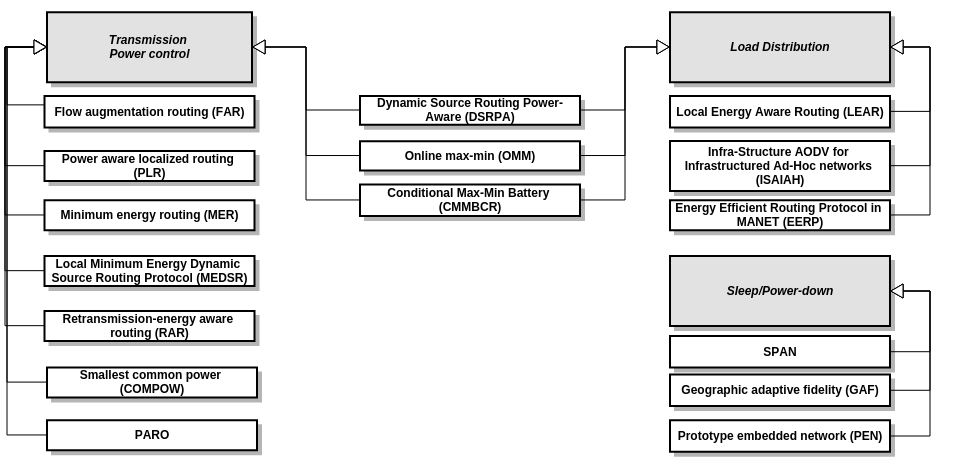
\includegraphics[width=0.9\textwidth]{images/overview}
  \caption{Overview of the protocols}
  
\end{figure}
\end{frame}
\begin{frame}{Online max-min (OMM)\cite{li2001online}}
\begin{block}{Metrics}
    \begin{enumerate}
        \item \textbf{min-power} The path requiring the least power
        \item \textbf{max-min} The path where the minimum of all nodes power levels after a transfer is maximal.
    \end{enumerate}
\end{block}

\begin{block}{How it works}
    \begin{itemize}
        \item Given a min-power path with power level $P_{min}$ and some constant $z \ge 1$:
         \begin{enumerate}
             \item  determine all paths with power levels less than $zP_{min}$
             \item choose the max-min path of those
         \end{enumerate}
        \item $z$ is random at the beginning, decreases unless expected lifetime of most used node increases if $z$ is (temporarily) increased
    \end{itemize}
\end{block}
\end{frame}
\begin{frame}{Online max-min (OMM)}
\begin{figure}
\centering
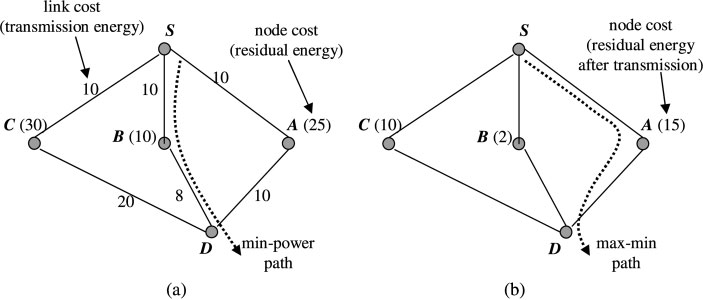
\includegraphics[width=\textwidth]{images/omm}
\caption{Paths in OMM\cite{alotaibi2012survey}}
\label{ommex}
\end{figure}
\end{frame}

\begin{frame}{Conditional max-min battery capacity routing (CMMBCR)\cite{toh2001maximum}}
    \begin{itemize}
        \item Similar to LEAR, OMM
        \item Pick a fixed threshold
        \item If all nodes in some paths have a higher energy level than the threshold, choose the min-power path
        \item Otherwise: Choose the max-min path
    \end{itemize}
\end{frame}

\begin{frame}{Dynamic Source Routing Power-Aware (DSRPA)\cite{djenouri2006new}}
    \begin{block}{Basics}
        \begin{itemize}
            \item Prefers paths with `fresh' batteries
            \item The more the difference in relative energy levels increases, the more prefer fresh batteries
        \end{itemize}
    \end{block}
    \begin{block}{Data dispersal}
        \begin{itemize}
            \item May distribute packets over optimal and less optimal paths
            \item Keep about twice the packets on a more optimal path than the next less-optimal one
            \item Helps reduce energy level differences
        \end{itemize}
    \end{block}
\end{frame}


\subsection{Sleep/Power-down}
\begin{frame}{Recap: Overview}
\begin{figure}
  \centering
  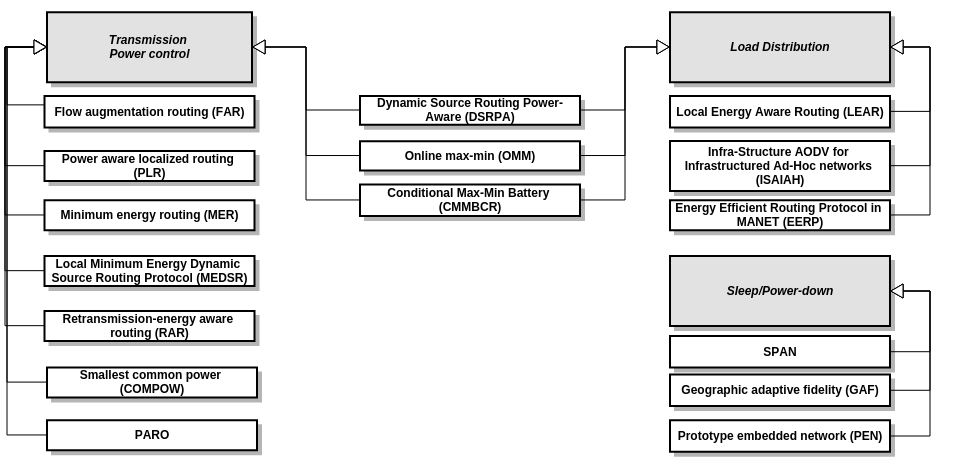
\includegraphics[width=0.9\textwidth]{images/overview}
  \caption{Overview of the protocols}
  
\end{figure}
\end{frame}

\begin{frame}{SPAN\cite{chen2002span}}
\begin{itemize}
    \item Master-slave protocols: A set of nodes picks a master to handle all forwarding duties
    \item Master $\leftrightarrow$ two neighbours cannot reach each other via 0, 1, or 2 masters
\end{itemize}
\begin{figure}
\centering
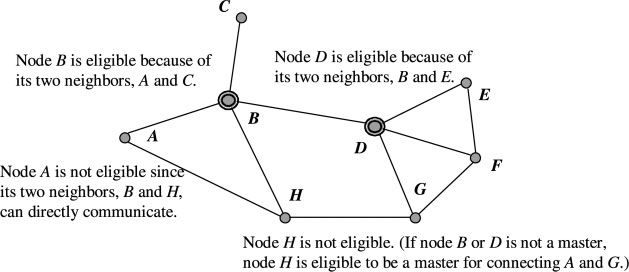
\includegraphics[width=0.7\textwidth]{images/span-master-example}
\caption{Master eligibility rule in the SPAN protocol\cite{alotaibi2012survey}}
\label{spanmaster}
\end{figure}

\end{frame}

\begin{frame}{Geographic adaptive fidelity (GAF)\cite{xu2001geography}}
    \begin{itemize}
        \item Group nodes into grids using geographic locations
        \item In each grid, node with highest energy level becomes master

    \end{itemize}
\label{gaf}
\begin{figure}[!t]
\subfloat[Grid example]{%
  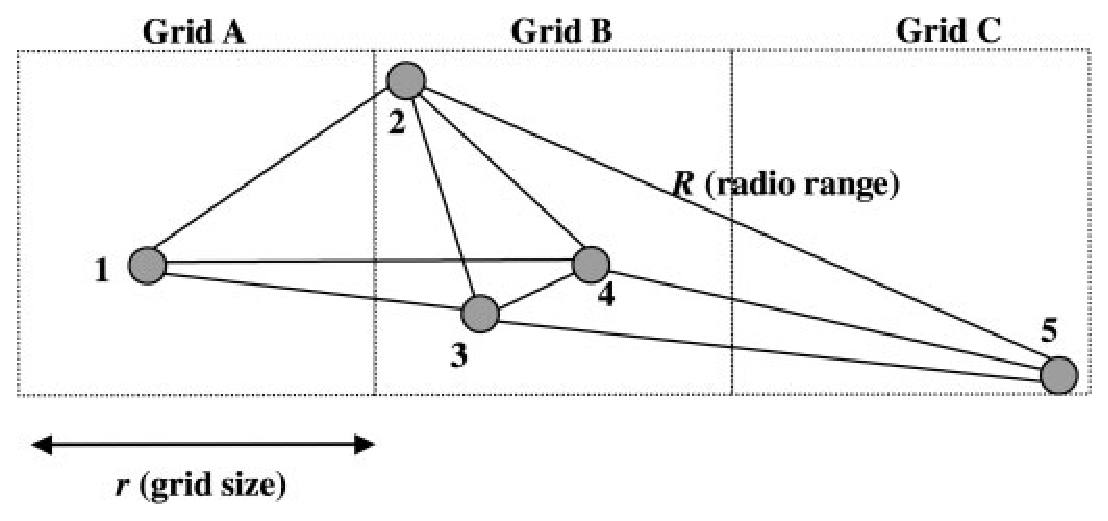
\includegraphics[width=0.46\textwidth]{images/gaf-grids}
  \label{gafgrids}
}
\hfill
\subfloat[Node states]{%
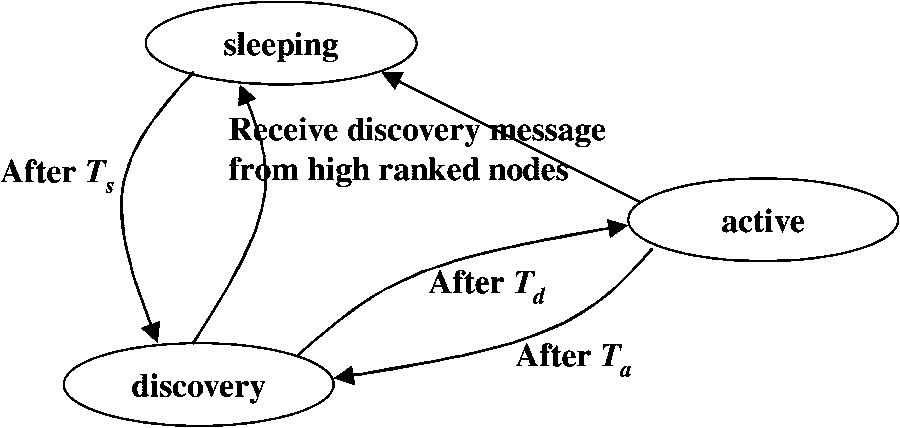
\includegraphics[width=0.46\textwidth]{images/gaf-states}
\label{gafstates}
}
\caption{Example grid and state diagram for GAF from \cite{alotaibi2012survey}}
\end{figure}
\end{frame}

\begin{frame}{Prototype embedded network (PEN)\cite{girling2000design}}

    \begin{block}{Transmitting}
    \begin{enumerate}
        \item Wait for broadcast from intended destination
        \item Send communication request
        \item Send data
    \end{enumerate}
    \end{block}
    \begin{block}{Receiving}
    Periodically wake up and
    \begin{enumerate}
        \item Advertise presence
        \item Listen for communication requests
        \item Process communication requests
    \end{enumerate}
    \end{block}
$\rightarrow$ No masters or slaves!
\end{frame}

\section{Summary}
\frame{\tableofcontents[currentsection]}
\begin{frame}{Summary}
\begin{itemize}
    \item Lots of use cases: Mobile phones, internet of things, sensors
    \item Many routing protocols
    \item Most routing protocols based on controlling transmission power
    \item A route with more hops might be more efficient than a route with less hops
    \item Can use geographic locations to optimise power usage
\end{itemize}
\end{frame}

\begin{frame}[allowframebreaks]
\frametitle{References}
\bibliographystyle{IEEEtran}
\bibliography{IEEEabrv,manets}
\end{frame}
\end{document}
